%beamer

% Comment/uncomment this line to toggle handout mode
%  \newcommand{\handout}{}

\ifdefined \handout
\documentclass[handout]{sdqbeamer} % Handout mode
\else
\documentclass{sdqbeamer}
\fi

%% UTF-8-Encoding
\usepackage[utf8]{inputenc}

% % \bigtimes abgeschrieben von http://tex.stackexchange.com/questions/14386/importing-a-single-symbol-from-a-different-font
% \DeclareFontFamily{U}{mathx}{\hyphenchar\font45}
% \DeclareFontShape{U}{mathx}{m}{n}{
%       <5> <6> <7> <8> <9> <10> gen * mathx
%       <10.95> mathx10 <12> <14.4> <17.28> <20.74> <24.88> mathx12
%       }{}
% \DeclareSymbolFont{mathx}{U}{mathx}{m}{n}
% \DeclareMathSymbol{\bigtimes}{\mathop}{mathx}{161}

\RequirePackage{xcolor}

\def\9{\square}
%\def\9{\blank}

% f"ur Aussagenlogik
\colorlet{alcolor}{blue}
\RequirePackage{tikz}
\usetikzlibrary{arrows.meta}
\newcommand{\alimpl}{\mathrel{\tikz[x={(0.1ex,0ex)},y={(0ex,0.1ex)},>={Classical TikZ Rightarrow[]}]{\draw[alcolor,->,line width=0.7pt,line cap=round] (0,0) -- (15,0);\path (0,-6);}}}
\newcommand{\alrimpl}{\mathrel{\tikz[x={(0.1ex,0ex)},y={(0ex,0.1ex)},>={Classical TikZ Leftarrow[]}]{\draw[alcolor,->,line width=0.7pt,line cap=round] (0,0) -- (15,0);\path (0,-6);}}}
\newcommand{\aleqv}{\mathrel{\tikz[x={(0.1ex,0ex)},y={(0ex,0.1ex)},>={Classical TikZ Rightarrow[]}]{\draw[alcolor,<->,line width=0.7pt,line cap=round] (0,0) -- (18,0);\path (0,-6);}}}
\newcommand{\aland}{\mathbin{\raisebox{-0.6pt}{\rotatebox{90}{\texttt{\color{alcolor}\char62}}}}}
\newcommand{\alor}{\mathbin{\raisebox{-0.8pt}{\rotatebox{90}{\texttt{\color{alcolor}\char60}}}}}
%\newcommand{\ali}[1]{_{\mathtt{\color{alcolor}#1}}}
\newcommand{\alv}[1]{\mathtt{\color{alcolor}#1}}
\newcommand{\alnot}{\mathop{\tikz[x={(0.1ex,0ex)},y={(0ex,0.1ex)}]{\draw[alcolor,line width=0.7pt,line cap=round,line join=round] (0,0) -- (10,0) -- (10,-4);\path (0,-8) ;}}}
\newcommand{\alvdash}{\mathrel{\tikz[x=4pt,y=3pt] {\draw[alcolor,line width=0.7pt,line cap=round,line join=round] (0,0) -- (0,1) -- (1,1) -- (0,1) -- (0,2);}}}
\newcommand{\alP}{\alv{P}} %ali{#1}}
\newcommand{\alQ}{\alv{Q}} %ali{#1}}
\newcommand{\alR}{\alv{R}} %ali{#1}}
\newcommand{\alS}{\alv{S}} %ali{#1}}
%\newcommand{\alka}{\negthinspace\hbox{\texttt{\color{alcolor}(}}}
\newcommand{\alka}{\negthinspace\text{\texttt{\color{alcolor}(}}}
%\newcommand{\alkz}{\texttt{\color{alcolor})}}\negthinspace}
\newcommand{\alkz}{\text{\texttt{\color{alcolor})}}\negthinspace}
\newcommand{\altrue}{\texttt{\textcolor{alcolor}{WAHR}}}
\newcommand{\alfalse}{\texttt{\textcolor{alcolor}{FALSCH}}}
\newcommand{\AAL}{A_{AL}}
\newcommand{\LAL}{\hbox{\textit{For}}_{AL}}
\newcommand{\AxAL}{\hbox{\textit{Ax}}_{AL}}
\newcommand{\AxEq}{\hbox{\textit{Ax}}_{Eq}}
\newcommand{\AxPL}{\hbox{\textit{Ax}}_{PL}}
\newcommand{\AALV}{\hbox{\textit{Var}}_{AL}}
\newcommand{\MP}{\hbox{\textit{MP}}}
\newcommand{\GEN}{\hbox{\textit{GEN}}}
\newcommand{\W}{\ensuremath{\hbox{\textbf{w}}}\xspace}
\newcommand{\F}{\ensuremath{\hbox{\textbf{f}}}\xspace}
\newcommand{\WF}{\ensuremath{\{\W,\F\}}\xspace}
\newcommand{\val}{\hbox{\textit{val}}}
\newcommand{\valDIb}{\val_{D,I,\beta}}

\newcommand*{\from}{\colon}

% die nachfolgenden Sachen angepasst an cmtt
\newlength{\ttquantwd}
\setlength{\ttquantwd}{1ex}
\newlength{\ttquantht}
\setlength{\ttquantht}{6.75pt}
\def\plall{%
  \tikz[line width=0.67pt,line cap=round,line join=round,baseline=(B),alcolor] {
    \draw (-0.5\ttquantwd,\ttquantht) -- node[coordinate,pos=0.4] (lll){} (-0.25pt,-0.0pt) -- (0.25pt,-0.0pt) -- node[coordinate,pos=0.6] (rrr){} (0.5\ttquantwd,\ttquantht);
    \draw (lll) -- (rrr);
    \coordinate (B) at (0,-0.35pt);
  }%
}
\def\plexist{%
  \tikz[line width=0.67pt,line cap=round,line join=round,baseline=(B),alcolor] {
    \draw (-0.9\ttquantwd,\ttquantht) -- (0,\ttquantht) -- node[coordinate,pos=0.5] (mmm){} (0,0) --  (-0.9\ttquantwd,0);
    \draw (mmm) -- ++(-0.75\ttquantwd,0);
    \coordinate (B) at (0,-0.35pt);
  }\ensuremath{\,}%
}
\let\plexists=\plexist
\newcommand{\NT}[1]{\ensuremath{\langle\mathrm{#1} \rangle}}

\newcommand{\CPL}{\text{\itshape Const}_{PL}}
\newcommand{\FPL}{\text{\itshape Fun}_{PL}}
\newcommand{\RPL}{\text{\itshape Rel}_{PL}}
\newcommand{\VPL}{\text{\itshape Var}_{PL}}
\newcommand{\ATer}{A_{\text{\itshape Ter}}}
\newcommand{\ARel}{A_{\text{\itshape Rel}}}
\newcommand{\AFor}{A_{\text{\itshape For}}}
\newcommand{\LTer}{L_{\text{\itshape Ter}}}
\newcommand{\LRel}{L_{\text{\itshape Rel}}}
\newcommand{\LFor}{L_{\text{\itshape For}}}
\newcommand{\NTer}{N_{\text{\itshape Ter}}}
\newcommand{\NRel}{N_{\text{\itshape Rel}}}
\newcommand{\NFor}{N_{\text{\itshape For}}}
\newcommand{\PTer}{P_{\text{\itshape Ter}}}
\newcommand{\PRel}{P_{\text{\itshape Rel}}}
\newcommand{\PFor}{P_{\text{\itshape For}}}

\newcommand{\plka}{\alka}
\newcommand{\plkz}{\alkz}
%\newcommand{\plka}{\plfoo{(}}
%\newcommand{\plkz}{\plfoo{)}}
\newcommand{\plcomma}{\hbox{\texttt{\color{alcolor},}}}
\newcommand{\pleq}{{\color{alcolor}\doteq}}

% MODIFIED (DJ)
% previously: \newcommand{\plfoo}[1]{\mathtt{\color{alcolor}#1}}
\newcommand{\plfoo}[1]{\texttt{\color{alcolor}#1}}

\newcommand{\plc}{\plfoo{c}}
\newcommand{\pld}{\plfoo{d}}
\newcommand{\plf}{\plfoo{f}}
\newcommand{\plg}{\plfoo{g}}
\newcommand{\plh}{\plfoo{h}}
\newcommand{\plx}{\plfoo{x}}
\newcommand{\ply}{\plfoo{y}}
\newcommand{\plz}{\plfoo{z}}
\newcommand{\plR}{\plfoo{R}}
\newcommand{\plS}{\plfoo{S}}

\newcommand{\bv}{\mathrm{bv}}
\newcommand{\fv}{\mathrm{fv}}

%\newcommand{\AxAL}{\hbox{\textit{Ax}}_{AL}}
%\newcommand{\AALV}{\hbox{\textit{Var}}_{AL}}

%\renewcommand{\#}[1]{\literal{#1}}
\newcommand{\A}{\mathcal{A}}
\newcommand{\Adr}{\text{Adr}}
\newcommand{\ar}{\mathrm{ar}}
\newcommand{\ascii}[1]{\literal{\char#1}}
%\newcommand{\assert}[1]{\text{/\!\!/\ } #1}
\newcommand{\assert}[1]{\colorbox{black!7!white}{\ensuremath{\{\;#1\;\}}}}
\newcommand{\Assert}[1]{$\langle$\textit{#1}$\rangle$}
\newcommand{\B}{\mathcal{B}}
\newcommand{\bfmod}{\mathbin{\kw{ mod }}}
\newcommand{\bb}{{\text{bb}}}
\def\bottom{\hbox{\small$\pmb{\bot}$}}
\newcommand{\card}[1]{|#1|}
%\newcommand{\cod}{\mathop{\text{cod}}}  % ist in thwmathabbrevs
\newcommand{\Conf}{\mathcal{C}}
\newcommand{\define}[1]{\emph{#1}}
%\renewcommand{\dh}{d.\,h.\@\xspace}
%\newcommand{\Dh}{D.\,h.\@\xspace}
%\newcommand{\engl}[1]{engl.\xspace\emph{#1}}
\newcommand{\eps}{\varepsilon}
%\newcommand{\evtl}{evtl.\@\xspace}
\newcommand{\fbin}{\text{bin}}
\newcommand{\finv}{\text{inv}}
\newcommand{\fnum}{\text{num}}
\newcommand{\fNum}{{\text{Num}}}
\newcommand{\frepr}{\text{repr}}
\newcommand{\fRepr}{\text{Repr}}
\newcommand{\fZkpl}{\text{Zkpl}}
\newcommand{\fLen}{\text{Len}}
\newcommand{\fsem}{\text{sem}}
\providecommand{\fspace}{\mathord{\text{space}}}
\providecommand{\fSpace}{\mathord{\text{Space}}}
\providecommand{\ftime}{\mathord{\text{time}}}
\providecommand{\fTime}{\mathord{\text{Time}}}
\newcommand{\fTrans}{\text{Trans}}
\newcommand{\fVal}{\text{Val}}

% MODIFIED (DJ)
\newcommand{\Val}{\text{Val}}

%\def\G{\mathbb{Z}}
\newcommand{\HT}[1]{\normalfont\textsc{HT-#1}}
\newcommand{\htr}[3]{\{#1\}\;#2\; \{#3\}}
\newcommand{\Id}{\text{I}}
%\newcommand{\ie}{i.\,e.\@\xspace}
\newcommand{\instr}[2]{\texttt{#1}\ \textit{#2}}
\newcommand{\Instr}[2]{\texttt{#1}\ \textrm{#2}}
\newcommand{\instrr}[3]{\texttt{#1}\ \textit{#2}\texttt{(#3)}}
\newcommand{\Instrr}[3]{\texttt{#1}\ \textrm{#2}\texttt{(#3)}}

% MODIFIED (DJ)
% previously:  \newcommand{\io}{\!\mid\!}
\newcommand{\io}{\ensuremath{\!\mid\!}}

%\usepackage{KITcolors}
\newcommand{\literal}[1]{\hbox{\textcolor{blue!95!white}{\textup{\texttt{\scalebox{1.11}{#1}}}}}}
%\newcommand{\literal}[1]{\hbox{\textcolor{KITblue!80!black}{\textup{\texttt{#1}}}}}
\def\kasten#1{\leavevmode\literal{\setlength{\fboxsep}{1pt}\fbox{\vrule  width 0pt height 1.5ex depth 0.5ex #1}}}
\newcommand{\kw}[1]{\ensuremath{\mathbf{#1}}}
\newcommand{\lang}[1]{\ensuremath{\langle#1\rangle}}
%\newcommand{\maw}{m.\,a.\,w.\@\xspace}
%\newcommand{\MaW}{M.\,a.\,w.\@\xspace}
\newcommand{\mdefine}[2][FOOBAR]{\define{#2}\def\foobar{FOOBAR}\def\optarg{#1}\ifx\foobar\optarg\def\optarg{#2}\fi\graffito{\optarg}}
\newcommand{\meins}{\rotatebox[origin=c]{180}{1}}
\newcommand{\Mem}{\text{Mem}}
\newcommand{\memread}{\text{memread}}
\newcommand{\memwrite}{\text{memwrite}}
\providecommand{\meta}[1]{\ensuremath{\langle}\textit{#1}\ensuremath{\rangle}}
%\newcommand{\N}{\mathbb{N}}
\newcommand{\NP}{\mathbf{NP}}
\newcommand{\Nadd}{N_{\text{add}}}
\newcommand{\Nmult}{N_{\text{mult}}}
% MODIFIED (DJ): added \!, mathcal{O}
\newcommand{\Oh}[1]{\mathcal{O}\!\left(#1\right)}
\newcommand{\Om}[1]{\Omega\!\left(#1\right)}
\newcommand{\personname}[1]{\textsc{#1}}
\newcommand{\regname}[1]{\texttt{#1}}
\newcommand{\mima}{\textsc{Mima}\xspace}
\newcommand{\mimax}{\textsc{Mima-X}\xspace}

\def\Pclass{\text{\bfseries P}}
\def\PSPACE{\text{\bfseries PSPACE}}

\newcommand{\SPush}{\text{push}}
\newcommand{\SPop}{\text{pop}}
\newcommand{\SPeek}{\text{peek}}
\newcommand{\STop}{\text{top}}
\newcommand{\STos}{\text{\itshape tos}}
\newcommand{\SBos}{\text{\itshape bos}}

%\newcommand{\R}{\mathbb{R}}
\newcommand{\Rnullplus}{\R_0^{+}}
\newcommand{\Rplus}{\R_{+}}
\newcommand{\resp}{resp.\@\xspace}
\newcommand{\Sem}{\text{Sem}}
\newcommand{\sgn}{\mathop{\text{sgn}}}
\newcommand{\sqbox}{\mathop{\raisebox{-6.2pt}{\hbox{\hbox to 0pt{$^{^{\sqcap}}$\hss}$^{^{\sqcup}}$}}}}
\newcommand{\sqleq}{\sqsubseteq}
\newcommand{\sqgeq}{\sqsupseteq}
% MODIFIED (DJ): added \!
\newcommand{\Th}[1]{\Theta\!\left(#1\right)}
%\newcommand{\usw}{usw.\@\xspace}
\newcommand{\V}[1]{\hbox{\textit{#1}}}
\newcommand{\x}{\times}
\newcommand{\ZK}{\mathbb{K}}
%\newcommand{\Z}{\mathbb{Z}}
\newcommand{\zB}{z.\,B.\@\xspace}
\newcommand{\ZB}{Z.\,B.\@\xspace}
% \newcommand{\bb}{{\text{bb}}}
% \def\##1{\hbox{\textcolor{darkblue}{\texttt{#1}}}}
% \def\A{\mathcal{A}}
% \newcommand{\0}{\#0}
% \newcommand{\1}{\#1}
% \newcommand{\Obj}{\text{Obj}}
% \newcommand{\start}{\mathop{\text{start}}}
% \newcommand{\compactlist}{\addtolength{\itemsep}{-\parskip}}
% \newcommand{\fval}{\text{val}}
% \newcommand{\lang}[1]{\ensuremath{\langle#1\rangle}}
% \newcommand{\io}{\!\mid\!}
% \def\sqbox{\mathop{\raisebox{-6.2pt}{\hbox{\hbox to 0pt{$^{^{\sqcap}}$\hss}$^{^{\sqcup}}$}}}}
% \def\sqleq{\sqsubseteq}
% \def\sqgeq{\sqsupseteq}
\def\Td{T_{\overline{d}}}
% \newcommand{\csym}[1]{\ensuremath{\#{c}_{\#{\hbox{\scriptsize #1}}}}}
% \newcommand{\F}{\ensuremath{\mathcal{F}}}
% \newcommand{\fsym}[2]{\ensuremath{\#{f}^{\#{\hbox{\scriptsize #1}}}_{\#{\hbox{\scriptsize #2}}}}}
% \newcommand{\rsym}[2]{\ensuremath{\#{R}^{\#{\hbox{\scriptsize #1}}}_{\#{\hbox{\scriptsize #2}}}}}
% \newcommand{\xsym}[1]{\ensuremath{\#{x}_{\#{\hbox{\scriptsize #1}}}}}
% \newcommand{\I}{\mathcal{I}}
% ********************************************************************
\usepackage{environ}
\usepackage{bm}
\usepackage{calc}
\usepackage{varwidth}
\usepackage{wasysym}
\usepackage{mathtools}


% Das ist der KIT-Stil
%\usepackage{../TutTexbib/beamerthemekit}
\titleimage{banner_2020_kit}
%\usetheme[deutsch,titlepage0]{KIT}

% Include PDFs
\usepackage{pdfpages}

% Libertine font (Original GBI font)
%\usepackage{libertine}
%\renewcommand*\familydefault{\sfdefault}  %% Only if the base font of the document is to be sans serif

% Nicer math symbols
\usepackage{eulervm}
%\usepackage{mathpazo}
\renewcommand\ttdefault{cmtt} % Computer Modern typewriter font, see lecture slides.

\usepackage{csquotes}

%%%%%%

%% Schönere Schriften
\usepackage[TS1,T1]{fontenc}

%% Bibliothek für Graphiken
\usepackage{graphicx}

%% der wird sowieso in jeder Datei gesetzt
\graphicspath{{../figures/}}

%% Anzeigetiefe für Inhaltsverzeichnis: 1 Stufe
\setcounter{tocdepth}{1}

%% Hyperlinks
\usepackage{hyperref}
% I don't know why, but this works and only includes sections and NOT subsections in the pdf-bookmarks.
\hypersetup{bookmarksdepth=subsection} 

%\usepackage{lmodern}
\usepackage{colortbl}
\usepackage[absolute,overlay]{textpos}
\usepackage{listings}
\usepackage{forloop}
%\usepackage{algorithmic} % PseudoCode package 

\usepackage{tikz}
\usetikzlibrary{matrix}
\usetikzlibrary{arrows.meta}
\usetikzlibrary{automata}
\usetikzlibrary{tikzmark}
\usetikzlibrary{positioning}

% Why has no-one come up with this yet? I mean, seriously. -.-
\tikzstyle{loop below right} = [loop, out=-60,in=-30, looseness=7]
\tikzstyle{loop below left} = [loop, out=-150,in=-120, looseness=7]
\tikzstyle{loop above right} = [loop, out=60,in=30, looseness=7]
\tikzstyle{loop above left} = [loop, out=150,in=120, looseness=7]
\tikzstyle{loop right below} = [loop below right]
\tikzstyle{loop left below} = [loop below left]
\tikzstyle{loop right above} = [loop above right]
\tikzstyle{loop left above} = [loop above left]

% Needed for gbi-macros
\usepackage{xspace}

%%%%%%

%% Verbatim
\usepackage{moreverb}

%%%%%%%%%%%%%%%%%%%%%%%%%%%%%%%%%%%% Copy end

%% Tabellen
\usepackage{array}
\usepackage{multicol}
\usepackage{hhline}

%% Bibliotheken für viele mathematische Symbole
\usepackage{amsmath, amsfonts, amssymb}

%% Deutsche Silbentrennung und Beschriftungen
\usepackage[ngerman]{babel}

%\usepackage{kbordermatrix}

% kbordermatrix settings
%\renewcommand{\kbldelim}{(} % Left delimiter
%\renewcommand{\kbrdelim}{)} % Right delimiter


% This is a configuration file with personal tutor information.
% It is therefore excluded from the git repository, so changes in this file will not conflict in git commits.

% Copy this template, rename to config.tex and add your information below.

\newcommand{\myname}{Lennart Rak}
\newcommand{\mymail}{lennart.rak@student.kit.edu} % Consider using your named student mail address to keep your u**** account private.
\newcommand{\mytutnumber}{02}

% Don't forget to update ILIAS url. WARNING: Underscores '_' and Ampersands '&' have to be escaped with backslashes '\'. Blame TeX, not me.
\newcommand{\myILIASurl}{http://s.kit.edu/gbi}

% Uncommenting this will print Socrative info with here defined roomname whenever \Socrative is called.
% (Otherwise, \Socrative will remain silent.)
% \newcommand{\mysocrativeroom}{???}

%\def\ThassesTut{}
\def\DanielsTut{}

\newcommand{\aboutMeFrame}{
	\begin{frame}{Über mich}
		\myname \\
		Informatik, 5. Fachsemester (Bachelor)
		
		% Lebensgeschichte...
		% Stammbaum...
		% Aufarbeitung der eigenen Todesser-Vergangenheit...
	\end{frame}
}
\newcommand{\aboutYouFrame}{
	\begin{frame}{Über euch}
	Wie heißt ihr? \\
	In welcher O-Phasen Gruppe wart ihr und was war euer Highlight? \\
	Habt ihr schon einen Partner zum Übungsblatt abgeben?
	    
	\end{frame}
}

\def\thisyear{2022}

% Update date of exam
\def\myKlausurtermin{27.~Februar~2023, 11:00–13:00~Uhr}

\def\mydate#1{
		  \ifnum#1=1\relax	  31. Oktober \thisyear \
	\else \ifnum#1=2\relax	  07. November \thisyear \
	\else \ifnum#1=3\relax    14. November \thisyear \
	\else \ifnum#1=4\relax    21. November \thisyear \
	\else \ifnum#1=5\relax    28. November \thisyear \
	\else \ifnum#1=6\relax    05. Dezember \thisyear \
	\else \ifnum#1=7\relax    12. Dezember \thisyear \
	\else \ifnum#1=8\relax    19. Dezember \thisyear \
	\else \ifnum#1=9\relax    09. Januar \thisyear \
	\else \ifnum#1=10\relax   16. Januar \nextyear \
	\else \ifnum#1=11\relax   23. Januar \nextyear \
	\else \ifnum#1=12\relax   30. Januar \nextyear \
	\else \ifnum#1=13\relax   06. Februar \nextyear \
	\else \ifnum#1=14\relax   13. Februar \nextyear \
	\else \textbf{Datum undefiniert!} 
	\fi\fi\fi\fi\fi\fi\fi\fi\fi\fi\fi\fi\fi\fi
}
\def\myshortdate#1{
		  \ifnum#1=1\relax	  31. 10 \thisyear \
	\else \ifnum#1=2\relax	  07. 11 \thisyear \
	\else \ifnum#1=3\relax    14. 11 \thisyear \
	\else \ifnum#1=4\relax    21. 11 \thisyear \
	\else \ifnum#1=5\relax    28. 11 \thisyear \
	\else \ifnum#1=6\relax    05. 12 \thisyear \
	\else \ifnum#1=7\relax    12. 12 \thisyear \
	\else \ifnum#1=8\relax    19. 12 \thisyear \
	\else \ifnum#1=9\relax    09. 01 \thisyear \
	\else \ifnum#1=10\relax   16. 01 \nextyear \
	\else \ifnum#1=11\relax   23. 01 \nextyear \
	\else \ifnum#1=12\relax   30. 01 \nextyear \
	\else \ifnum#1=13\relax   06. 02 \nextyear \
	\else \ifnum#1=14\relax   13. 02 \nextyear \
	\else \textbf{Datum undefiniert!} 
	\fi\fi\fi\fi\fi\fi\fi\fi\fi\fi\fi\fi\fi\fi
}

\def\mylasttimestext{Was bisher geschah...}

\colorlet{beamerlightred}{red!40}
\colorlet{beamerlightgreen}{green!50}
\colorlet{beamerlightyellow}{yellow!50}
\colorlet{lightred}{red!30}
\colorlet{lightgreen}{green!40}
\colorlet{lightyellow}{yellow!50}
\colorlet{fullred}{red!60}
\colorlet{fullgreen}{green}

\definecolor{myalertcolor}{rgb}{1,0.33,0.24}
\setbeamercolor{alerted text}{fg=myalertcolor}

% Flag to toggle display of KIT Logo.
% If you want to conform to the official logo guidelines, 
% you are not allowed to use the logo and should disable it
% using the following flag. Just saying.
% (But it's too beautiful, so best leave this commented. :P)
\newcommand{\noKITLogo}{}

% Toggle handout mode by including the following line before including PraeambelTut
% and removing the % at the start (but do NOT remove the % char here, otherwise handout mode will always be on!)
% Please keep handout mode off in all commits!

% \newcommand{\handout}{}



% define custom \handout command flag if handout mode is toggled  #DirtyAsHellButWell...
\only<beamer:0>{\def\handout{}} %beamer:0 == handout mode

\newcommand{\R}{\mathbb{R}}
\newcommand{\N}{\mathbb{N}}
\newcommand{\Z}{\mathbb{Z}}
\newcommand{\Q}{\mathbb{Q}}
\newcommand{\BB}{\mathbb{B}}
\newcommand{\C}{\mathbb{C}}
\newcommand{\K}{\mathbb{K}}
\newcommand{\G}{\mathbb{G}}
\newcommand{\nullel}{\mathcal{O}}
\newcommand{\einsel}{\mathds{1}}
\newcommand{\Pot}{\mathcal{P}}
\renewcommand{\O}{\text{O}}

\def\word#1{\hbox{\textcolor{blue}{\texttt{#1}}}}
\let\literal\word
\def\mword#1{\hbox{\textcolor{blue}{$\mathtt{#1}$}}}  % math word
\def\sp{\scalebox{1}[.5]{\textvisiblespace}}
\def\wordsp{\word{\sp}}

%\newcommand{\literal}[1]{\textcolor{blue}{\texttt{#1}}}
\newcommand{\realTilde}{\textasciitilde \ }
\newcommand{\setsize}[1]{\ensuremath{\left\lvert #1 \right\rvert}}
\newcommand{\size}[1]{\setsize{#1}}  % Shame on you, TeXStudio...
\newcommand{\set}[1]{\left\{#1\right\}}
\newcommand{\tuple}[1]{\left(#1\right)}
\newcommand{\normalvar}[1]{\text{$#1$}}

% Modified by DJ
\let\oldemptyset\emptyset
\let\emptyset\varnothing % proper emptyset

\newcommand{\boder}{\ensuremath{\mathbin{\textcolor{blue}{\vee}}}\xspace}
\newcommand{\bund}{\ensuremath{\mathbin{\textcolor{blue}{\wedge}}}\xspace}
\newcommand{\bimp}{\ensuremath{\mathrel{\textcolor{blue}{\to}}}\xspace}
\newcommand{\bgdw}{\ensuremath{\mathrel{\textcolor{blue}{\leftrightarrow}}}\xspace}
\newcommand{\bnot}{\ensuremath{\textcolor{blue}{\neg}}\xspace}
\newcommand{\bone}{\ensuremath{\textcolor{blue}{1}}\text{}}
\newcommand{\bzero}{\ensuremath{\textcolor{blue}{0}}\text{}}
\newcommand{\bleftBr}{\ensuremath{\textcolor{blue}{\texttt{(}}}\text{}}
\newcommand{\brightBr}{\ensuremath{\textcolor{blue}{\texttt{)}}}\text{}}

% Fix of \b... commands:

\renewcommand{\boder}{\alor}
\renewcommand{\bund}{\aland}
\renewcommand{\bimp}{\alimpl}
\renewcommand{\bgdw}{\aleqv}
\renewcommand{\bnot}{\alnot}
\renewcommand{\bleftBr}{\alka}
\renewcommand{\brightBr}{\alkz}
\newcommand{\alA}{\word A}
\newcommand{\alB}{\word B}
\newcommand{\alC}{\word C}

\newcommand{\plB}{\plfoo{B}}
\newcommand{\plE}{\plfoo{E}}

\newcommand{\summe}[2]{\sum\limits_{#1}^{#2}}
\newcommand{\limes}[1]{\lim\limits_{#1}}

%\newcommand{\numpp}{\advance \value{weeknum} by -2 \theweeknum \advance \value{weeknum} by 2}
%\newcommand{\nump}{\advance \value{weeknum} by -1 \theweeknum \advance \value{weeknum} by 1}

\newcommand{\mycomment}[1]{}
\newcommand{\Comment}[1]{}

%% DISCLAIMER START 
% It is INSANELY IMPORTANT NOT TO DO THIS OUTSIDE BEAMER CLASS! IN ARTCILE DOCUMENTS, THIS IS VERY LIKELY TO BUG AROUND!
\makeatletter%
\@ifclassloaded{beamer}%
{
	% TODO 
	% no time... later.   (= never -.-)
	% redefine section to ignore multiple \section calls with the same title
}%
{
	\errmessage{ERROR: section command redefinition outside of beamer class document! Please contact the author of this code or read the F-ing disclaimer.}
}%
\makeatother%
%% DISCLAIMER END

\newcounter{abc}
\newenvironment{alist}{
  \begin{list}{(\alph{abc})}{
      \usecounter{abc}\setlength{\leftmargin}{8mm}\setlength{\labelsep}{2mm}
    }
}{\end{list}}


\newcommand{\stdarraystretch}{1.20}
\renewcommand{\arraystretch}{\stdarraystretch}  % for proper row spacing in tables

\newcommand{\morescalingdelimiters}{   % for proper \left( \right) typography
	\delimitershortfall=-1pt  
	\delimiterfactor=1
}

\newcommand{\centered}[1]{\vspace{-\baselineskip}\begin{center}#1\end{center}\vspace{-\baselineskip}}

% for \implitem and \item[bla] stuff to look right:
\setbeamercolor*{itemize item}{fg=black}
\setbeamercolor*{itemize subitem}{fg=black}
\setbeamercolor*{itemize subsubitem}{fg=black}

\setbeamercolor*{description item}{fg=black}
\setbeamercolor*{description subitem}{fg=black}
\setbeamercolor*{description subsubitem}{fg=black}

\renewcommand{\qedsymbol}{\textcolor{black}{\openbox}}

\renewcommand{\mod}{\mathop{\textbf{mod}}}
\renewcommand{\div}{\mathop{\textbf{div}}}

\newcommand{\ceil}[1]{\left\lceil#1\right\rceil}
\newcommand{\floor}[1]{\left\lfloor#1\right\rfloor}
\newcommand{\abs}[1]{\left\lvert #1 \right\rvert}
\newcommand{\Matrix}[1]{\begin{pmatrix} #1 \end{pmatrix}}
\newcommand{\braced}[1]{\left\lbrace #1 \right\rbrace}

% "something" placeholder. Useful for repairing spacing of operator sections, like `\sth = 42`.
\def\sth{\vphantom{.}}

\def\fract#1/#2 {\frac{#1}{#2}} % ! Trailing space is crucial!
\def\dfract#1/#2 {\dfrac{#1}{#2}} % ! Trailing space is crucial!

\newcommand{\Mid}{\;\middle|\;}

\let\after\circ



\def\·{\cdot}
\def\*{\cdot}
\def\?>{\ensuremath{\rightsquigarrow}}  % Fuck you, Latex
\def\~~>{\ensuremath{\rightsquigarrow}}  

\newcommand{\tight}[1]{{\renewcommand{\arraystretch}{0.76} #1}}
\newcommand{\stackedtight}[1]{\renewcommand{\arraystretch}{0.76} \begin{matrix} #1 \end{matrix} }
\newcommand{\stacked}[1]{\begin{matrix} #1 \end{matrix} }
\newcommand{\casesl}[1]{\delimitershortfall=0pt  \left\lbrace\hspace{-.3\baselineskip}\begin{array}{ll} #1 \end{array}\right.}
\newcommand{\casesr}[1]{\delimitershortfall=0pt  \left.\begin{array}{ll} #1 \end{array}\hspace{-.3\baselineskip}\right\rbrace}
\newcommand{\caseslr}[1]{\delimitershortfall=0pt  \left\lbrace\hspace{-.3\baselineskip}\begin{array}{ll} #1 \end{array}\hspace{-.3\baselineskip}\right\rbrace}

\def\q#1uad{\ifnum#1=0\relax\else\quad\q{\the\numexpr#1-1\relax}uad\fi}
% e.g. \q1uad = \quad, \q2uad = \qquad etc.

\newcommand{\qqquad}{\q3uad}
\newcommand{\minusquad}{\hspace{-1em}}

%% Placeholder utils
% \§{#1}   Saves #1 as placeholder and prints it
% \.       Prints an \hphantom with the size of the recalled placeholder.
\def\indentstring{}
\def\§#1{\def\indentstring{#1}#1}
\def\.{{$\hphantom{\text{\indentstring}}$}}
%% Placeholder utils end

\newcommand{\impl}{\ifmmode\ensuremath{\mskip\thinmuskip\Rightarrow\mskip\thinmuskip}\else$\Rightarrow$\fi\xspace}
\newcommand{\Impl}{\ifmmode\implies\else$\Longrightarrow$\fi\xspace}

\newcommand{\derives}{\Rightarrow}

\newcommand{\gdw}{\ifmmode\mskip\thickmuskip\Leftrightarrow\mskip\thickmuskip\else$\Leftrightarrow$\fi\xspace}
\newcommand{\Gdw}{\ifmmode\iff\else$\Longleftrightarrow$\fi\xspace}

% Legacy code from the algo tutorial slides. Perhaps useful. Try with care.
\mycomment{
	\newcommand{\impl}{\ifmmode\ensuremath{\mskip\thinmuskip\Rightarrow\mskip\thinmuskip}\else$\Rightarrow$\xspace\fi}  
	\newcommand{\Impl}{\ifmmode\implies\else$\Longrightarrow$\xspace\fi}
	
	\newcommand{\gdw}{\ifmmode\mskip\thickmuskip\Leftrightarrow\mskip\thickmuskip\else$\Leftrightarrow$\xspace\fi}
	\newcommand{\Gdw}{\ifmmode\iff\else$\Longleftrightarrow$\xspace\fi}
}
	
\newcommand{\gdwdef}{\ifmmode\mskip\thickmuskip:\Leftrightarrow\mskip\thickmuskip\else:$\Leftrightarrow$\xspace\fi}
\newcommand{\Gdwdef}{\ifmmode\mskip\thickmuskip:\Longleftrightarrow\mskip\thickmuskip\else:$\Longleftrightarrow$\xspace\fi}

\newcommand{\symbitemnegoffset}{\hspace{-.5\baselineskip}}
\newcommand{\implitem}{\item[\impl\symbitemnegoffset]}
\newcommand{\Implitem}{\item[\Impl\symbitemnegoffset]}


\newcommand{\forcenewline}{\mbox{}\\}

\newcommand{\bfalert}[1]{\textbf{\alert{#1}}}
\let\elem\in   % I'm a Haskell freak. Don't judge me. :P


\def\|#1|{\text{\normalfont #1}}  % | steht für senkrecht (anstatt kursiv wie sonst im math mode)


% proper math typography
\newcommand{\functionto}{\longrightarrow}
\renewcommand{\geq}{\geqslant}
\renewcommand{\leq}{\leqslant}
\let\oldsubset\subset
\renewcommand{\subset}{\subseteq} % for all idiots out there using subset

\newenvironment{threealign}{%
	\[
	\begin{array}{r@{\ }c@{\ }l}
}{%
	\end{array}	
	\]
}

\newcommand{\concludes}{ \\ \hline  }
\newcommand{\deduction}[1]{
	\begin{varwidth}{.8\linewidth}
		\begin{tabular}{>{$}c<{$}}
			#1
		\end{tabular}
	\end{varwidth}	
}

\definecolor{hoareorange}{rgb}{1,.85,.6}
\newcommand{\hoareassert}[1]{\setlength{\fboxsep}{1pt}\setlength{\fboxrule}{-1.4pt}\fcolorbox{white}{hoareorange}{\ensuremath{\{\;#1\;\}}}\setlength\fboxrule{\defaultfboxrule}\setlength{\fboxsep}{3pt}}

\newcommand{\mailto}[1]{\href{mailto:#1}{{\textcolor{blue}{\underline{#1}}}}}
\newcommand{\urlnamed}[2]{\href{#2}{\textcolor{blue}{\underline{#1}}}}
\renewcommand{\url}[1]{\urlnamed{#1}{#1}}

\newcommand{\hanging}{\hangindent=0.7cm}
\newcommand{\indented}{\hanging}


% \hstretchto prints #2 left-aligned into a box of the width of #1
\def\hstretchto#1#2{%
	\mbox{}\vphantom{#2}\rlap{#2}\hphantom{#1}%
}

\def\vstretchto#1#2{%
	\mbox{}\hphantom{#2}\smash{#2}\vphantom{#1}%
}

% \hstretchtocentered prints #2 centered into a box of the width of #1
\def\hstretchtocentered#1#2{%
	\mbox{}\vphantom{#2}\scalebox{0.5}{\hphantom{#1}}\clap{#2}\scalebox{0.5}{\hphantom{#1}}%
}

% vertical centering
\newcommand{\vertcenter}[1]{%
	\ensuremath{\vcenter{\hbox{#1}}}%
}


%requires \thisyear to be defined (s. config.tex)!
\edef\nextyear{\the\numexpr\thisyear+1\relax}


% --- \frameheight constant ---
\newlength\fullframeheight
\newlength\framewithtitleheight
\setlength\fullframeheight{.92\textheight}
\setlength\framewithtitleheight{.86\textheight}

\newlength\frameheight
\setlength\frameheight{\fullframeheight}

\let\frametitleentry\relax
\let\oldframetitle\frametitle
\def\newframetitle#1{\global\def\frametitleentry{#1}\if\relax\frametitleentry\relax\else\setlength\frameheight{\framewithtitleheight}\fi\oldframetitle{#1}}
\let\frametitle\newframetitle

\def\newframetitleoff{\let\frametitle\oldframetitle}
\def\newframetitleon{\let\frametitle\newframetitle}
% --- \frameheight constant end ---

\newcommand{\fakeframetitle}[1]{%
	\vspace{-2.05\baselineskip}%
	{\Large \textbf{#1}} \\%
	\smallskip
}



\newenvironment{headframe}{\Huge THIS IS AN ERROR. PLEASE CONTACT THE ADMIN OF THIS TEX CODE. (headframe env def failed)}{}
\RenewEnviron{headframe}[1][]{
	\begin{frame}\frametitle{\ }
		\centering
		\Huge\textbf{\textsc{\BODY} \\
		}
		\Large {#1}
		\frametitle{\ }
	\end{frame}
}


\makeatletter
% Provides color if undefined.
\newcommand{\colorprovide}[2]{%
	\@ifundefinedcolor{#1}{\colorlet{#1}{#2}}{}}
\makeatother


\colorprovide{lightred}{red!30}
\colorprovide{lightgreen}{green!40}
\colorprovide{lightyellow}{yellow!50}
\colorprovide{lightblue}{blue!10}
\colorprovide{beamerlightred}{lightred}
\colorprovide{beamerlightgreen}{lightgreen}
\colorprovide{beamerlightyellow}{lightyellow}
\colorprovide{beamerlightblue}{lightblue}
\colorprovide{fullred}{red!60}
\colorprovide{fullgreen}{green}
\definecolor{darkred}{RGB}{115,48,38}
\definecolor{darkgreen}{RGB}{48,115,38}
\definecolor{darkyellow}{RGB}{100,100,0}

\only<handout:0>{\colorlet{adaptinglightred}{beamerlightred}}
\only<handout:0>{\colorlet{adaptinglightgreen}{beamerlightgreen}}
\only<handout:0>{\colorlet{adaptinglightyellow}{beamerlightyellow}}
\only<handout:0>{\colorlet{adaptinglightblue}{beamerlightblue}}
\only<beamer:0>{\colorlet{adaptinglightred}{lightred}}
\only<beamer:0>{\colorlet{adaptinglightgreen}{lightgreen}}
\only<beamer:0>{\colorlet{adaptinglightyellow}{lightyellow}}
\only<beamer:0>{\colorlet{adaptinglightblue}{lightblue}}
\only<handout:0>{\colorlet{adaptingred}{lightred}}
\only<beamer:0>{\colorlet{adaptingred}{fullred}}
\only<handout:0>{\colorlet{adaptinggreen}{lightgreen}}
\only<beamer:0>{\colorlet{adaptinggreen}{fullgreen}}



\newcommand{\TrueQuestion}[1]{
	\TrueQuestionE{#1}{}
}

\newcommand{\YesQuestion}[1]{
	\YesQuestionE{#1}{}
}

\newcommand{\FalseQuestion}[1]{
	\FalseQuestionE{#1}{}
}

\newcommand{\NoQuestion}[1]{
	\NoQuestionE{#1}{}
}

\newcommand{\DependsQuestion}[1]{
	\DependsQuestionE{#1}{}
}

\newcommand{\QuestionVspace}{\vspace{4pt}}
\newcommand{\QuestionParbox}[1]{\begin{varwidth}{.85\linewidth}#1\end{varwidth}}
\newcommand{\ExplanationParbox}[1]{\begin{varwidth}{.97\linewidth}#1\end{varwidth}}
\colorlet{questionlightgray}{gray!23}
\let\defaultfboxrule\fboxrule

% #1: bg color
% #2: fg color short answer
% #3: short answer text
% #4: question
% #5: explanation
\newcommand{\GenericQuestion}[5]{
	\setlength\fboxrule{2pt}
	\only<+|handout:0>{\hspace{-2pt}\fcolorbox{white}{questionlightgray}{\QuestionParbox{#4} \quad\textbf{?}}}
	\visible<+->{\hspace{-2pt}\fcolorbox{white}{#1}{\QuestionParbox{#4} \quad\textbf{\textcolor{#2}{#3}}} \if\relax#5\relax\else\ExplanationParbox{#5}\fi} \\
	\setlength\fboxrule{\defaultfboxrule}
}

% #1: Q text
% #2: Explanation
\newcommand{\TrueQuestionE}[2]{
	\GenericQuestion{adaptinglightgreen}{darkgreen}{Wahr.}{#1}{#2}
}

% #1: Q text
% #2: Explanation
\newcommand{\YesQuestionE}[2]{
	\GenericQuestion{adaptinglightgreen}{darkgreen}{Ja.}{#1}{#2}
}

% #1: Q text
% #2: Explanation
\newcommand{\FalseQuestionE}[2]{
	\GenericQuestion{adaptinglightred}{darkred}{Falsch.}{#1}{#2}
}

% #1: Q text
% #2: Explanation
\newcommand{\NoQuestionE}[2]{
	\GenericQuestion{adaptinglightred}{darkred}{Nein.}{#1}{#2}
}

% #1: Q text
% #2: Explanation
\newcommand{\DependsQuestionE}[2]{
	\GenericQuestion{adaptinglightyellow}{darkyellow}{Je nachdem!}{#1}{#2}
}

% #1: Q text
% #2: Answer
\newcommand{\ContentQuestion}[2]{
	\GenericQuestion{adaptinglightblue}{black}{\minusquad}{#1}{#2}
}

%\ifnum\thisyear=2018 \else \errmessage{Old ILIAS link inside preamble. Please update.} \fi

\newcommand{\ILIAS}{\urlnamed{ILIAS}{\myILIASurl}\xspace}
\newcommand{\Klausurtermin}{\myKlausurtermin\xspace}

\newcommand{\Socrative}{\ifdefined\mysocrativeroom \only<handout:0>{socrative.com $\quad \~~> \quad $ Student login \\ Raumname:  \mysocrativeroom\\ \medskip}\else\fi}

\newcommand{\thasse}[1]{
	\ifdefined\ThassesTut #1\xspace \else\fi
}
\newcommand{\daniel}[1]{
	\ifdefined\DanielsTut #1\xspace \else\fi
}
\newcommand{\thassedaniel}[2]{\ifdefined\ThassesTut #1\else\ifdefined\DanielsTut #2\fi\fi\xspace}

\ifdefined\ThassesTut \ifdefined\DanielsTut \errmessage{ERROR: Both ThassesTut and DanielsTut flags are set. This is most likely an error. Please check your config.tex file.} \else \fi \else \ifdefined\DanielsTut \else \errmessage{ERROR: Neither ThassesTut  nor DanielsTut flags are set. This is most likely an error. Please check your config.tex file.} \fi\fi

%\newcommand{\sgn}{\text{sgn}}

%%%%%%%%%%%% INHALT %%%%%%%%%%%%%%%%

%% Wochennummer
\newcounter{weeknum}

%% Titelinformationen
\title[GBI-Tutorium \mytutnumber, Woche \theweeknum]{Grundbegriffe der Informatik Tutorium \mytutnumber}

\subtitle{Woche \theweeknum \xspace}
\author[\myname]{\myname \xspace \normalfont (\mailto{\mymail})}
\groupname{KIT -- Karlsruher Institut für Technologie}
\date[\myshortdate{\theweeknum}]{\mydate{\theweeknum}}

% Modified, DJ (better safe than sorry)
%\AuthorTitleSep{ – }

%% Titel einfügen
\newcommand{\titleframe}{\KITtitleframe}

%% Alles starten mit \starttut{X}
\newcommand{\starttut}[1]{\setcounter{weeknum}{#1}\pdfinfo{
		/Author (\myname)
		/Title  (GBI-Tutorium \mytutnumber, Woche \theweeknum)
	}\titleframe\frame{\frametitle{Inhalt}\tableofcontents} \AtBeginSection[]{%
		\begin{frame}{Wo sind wir gerade?}
		\tableofcontents[currentsection]
	\end{frame}\addtocounter{framenumber}{-1}}}


\newcommand{\framePrevEpisode}{
\begin{headframe}
	\mylasttimestext
\end{headframe}
}

\newcommand{\lastframetitled}[6]{
% 	\frame{\frametitle{#6}
% 		\vspace{-#2\baselineskip}
% 		\begin{figure}[H]
% 			\centering
% 			\LARGE \textbf{\textsc{#5}} \\
% 			\vspace{.2\baselineskip}
% 			\includegraphics[#1]{#3}
% 			\vspace{-6pt}
% 			\begin{center}
% 				\small \url{#4} 
% 			\end{center}
% 		\end{figure} 
% 	}
\begin{frame}[plain]
    \vspace{\baselineskip}
    \centering
    \Large\textbf{#6}
    \begin{figure}[H]
		\centering
% 		\LARGE \textbf{\textsc{#5}} \\
% 		\vspace{.2\baselineskip}
		\includegraphics[#1]{#3}
		\vspace{-6pt}
		\begin{center}
			\small \url{#4} 
		\end{center}
	\end{figure}
\end{frame}
}

% #1 number
% #2 title 
% #3 vspace (positive) without unit (\baselineskip)
\newcommand{\xkcdframe}[3]{
	\lastframetitled{width=.96\textwidth}{#3}{xkcd/#1}{http://xkcd.com/#1}{}{#2}
}

\newcommand{\xkcdframevert}[3]
{
	\lastframetitled{height=.96\frameheight}{#3}{xkcd/#1}{http://xkcd.com/#1}{}{#2}
}

% #1 number
% #2 title 
% #3 vspace (positive) without unit (\baselineskip)
% #4 \includegraphics[] optional parameters
\newcommand{\xkcdframecustom}[4]
{
	\lastframetitled{#4}{#3}{xkcd/#1}{http://xkcd.com/#1}{}{#2}
}

\newcommand{\slideThanks}{
	\begin{frame}
	\frametitle{Credits}
	\begin{block}{}
		An der Erstellung des Foliensatzes haben mitgewirkt:\\[1em]
		Daniel Jungkind \\
		Thassilo Helmold \\
		Philipp Basler \\
		Nils Braun \\
		Dominik Doerner \\
		Ou Yue \\
	\end{block}
\end{frame}
}

%% Wörter DEPRECATED! DO NOT USE
\newcommand{\code}[1]{$\mathbf{#1}$}

\morescalingdelimiters

\begin{document}
\starttut{2}

\mycomment{
	Hier einmal Beweise und Gegenbeweise erklären damit die Tutanden
	es leichter haben das erste Übungsblatt zu lösen.
}

\Comment{
\begin{frame}{Organisatorisches}
	
	
		\begin{itemize}
	    \item Nächsten Donnerstag: Abgabe des ersten Übungsblattes! (Achtung: Bei nachfolgenden Blättern müsst ihr euch selber erinnern!)
		\end{itemize}
	
\end{frame}
\begin{frame}{Zu Blatt \#1}
	\begin{itemize}[<+->]
		\item Erstmal: Volle Punktzahl ist utopisch. Fehler macht man, um draus zu lernen – dazu sind ÜBs da
		\item Nicht mehrere Alternativen angeben, unter denen ich mir die richtige heraussuchen soll. (That's \emph{your} job!)
	\end{itemize}
\end{frame}

\begin{frame}[t]{Übungsblätter: Häufige Fehler \daniel{und anderer Kram}}
	
	\TrueQuestionE{Beweise fängt man mit der Behauptung an.}{}
	\FalseQuestionE{Wenn wir $A$ schreiben, ist das immer eine Menge, \\ und $f, g$ sind immer Funktionen.}{Das muss man \textbf{explizit} angeben.}
	\FalseQuestionE{Ein Beispiel langt als Beweis.}{...bis ein anderes Beispiel herkommt, bei dem es kaputt geht... \\
		\impl eine Behauptung \textbf{widerlegen} geht mit nem Beispiel sehr gut!}
	%Mit einem Beispiel kann man eine Behauptung widerlegen, es zeigt aber nicht die Allgemeingültigkeit}

	
	\medskip
	
	\uncover<8->{Passt auf, was eure Variablen sind und welche Operationen ihr darauf anwenden könnt. Mengen kann man nicht mit $\bund$ und $\boder$ verknüpfen und auch keine \impl dazwischen tun.}
	
\end{frame}
}


\framePrevEpisode

\begin{frame}{Wahr oder falsch?}
	\Socrative
	\TrueQuestionE{$ \setsize{\emptyset} = 0$.}{}
	\FalseQuestionE{$ \setsize{ \set{\set{}} } = 0$.}{$ \setsize{\set{\set{}}} = \setsize{\set{\emptyset}} = 1$.}
	\TrueQuestionE{$ \setsize{\set{ 1, \set{2, 3}, 4, \set{5,6,7}}} = 4$.}{$\set{2, 3}$ und $\set{5,6,7}$ sind zwei einzelne Objekte!}
	\TrueQuestionE{$ \{1, 2\} = \{2, 1\}$.}{}
	\FalseQuestion{$ (1, 2) = (2, 1)$.}
	\FalseQuestionE{$ \left(M\cup A\right)\setminus M = A $.}{für z.~B. $ M = A = \{1\}$}
	%TODO Relationen-Fragen noch? Wenn's im ersten Tut schon vorkam!
	\visible<12->{
	\begin{block}{Bemerkungen}
		Menge / Tupel: Klammern beachten! Einfache Beispiele helfen!
	\end{block}
	}
\end{frame}
\begin{frame}[t]{Wahr oder Falsch?}
	\FalseQuestionE{Eine Funktion muss linkseindeutig sein.}{\impl Eine Funktion muss rechtseindeutig \textbf{und linkstotal} sein.}
	\TrueQuestion{Eine injektive Funktion ist linkseindeutig.}
	\TrueQuestion{Eine surjektive Funktion ist rechtstotal.}
	\FalseQuestion{Jede Relation ist eine Funktion.}
	\TrueQuestion{Jede Funktion ist eine Relation.}
\end{frame}



\section{Relationen}
\begin{frame}{Relation}
  \begin{block}{Relation}
	Eine \emph{Relation} $R$ ist eine Teilmenge eines kartesischen Produkts, also $R \subseteq A \times B$. \\
  \end{block}
\end{frame}




\begin{frame}{Eigenschaften von Relationen}
  \begin{block}{Linkstotal}
	Eine Relation $R$ heißt \emph{linkstotal}, wenn es für jedes $a \in A$ \emph{mindestens} ein $b \in B$ gibt. \\
	\glqq \hspace{1pt}Von jedem Element in A geht mindestens ein Pfeil nach B.\grqq
  \end{block}
  \begin{figure}
    \begin{minipage}{0.44\textwidth}
      \centering
      \begin{tikzpicture}[x={(12mm,0mm)},y={(0mm,-5mm)}]
        \tikzset{
          blob/.style={circle,fill,minimum size=0.7mm,inner sep=0,outer sep=0}
        }
        \tikzset{
          rahmen/.style={draw,inner sep=3mm,rounded corners=2mm}
        }
        \tikzset{
          pfeil/.style={shorten >=0.1mm,shorten <=1mm,thick,-latex}
        }

        \node[blob]  (Al) at (0,0) {};
        \node[blob]  (Bl) at (0,1) {};
        \node[blob]  (Cl) at (0,2) {};
        \node[rahmen,fit=(Al) (Bl) (Cl)] {};
        \node at ($ (Al) + (0,-1.3) $) {$A$};

        \node[blob]  (Ar) at (1,0) {};
        \node[blob]  (Br) at (1,1) {};
        \node[blob]  (Cr) at (1,2) {};
        \node[rahmen,fit=(Ar) (Br) (Cr)] {};
        \node at ($ (Ar) + (0,-1.3) $) {$B$};

        \draw[pfeil] (Al) -- (Br);
        \draw[pfeil] (Bl) -- (Cr);

        \draw[red,line width=0.7mm,opacity=0.9] (Cl) -- +(-1.5mm,-1.5mm) (Cl)
  -- ++(1.5mm,-1.5mm)
        (Cl) -- ++(-1.5mm,1.5mm) (Cl) -- ++(1.5mm,1.5mm);
      \end{tikzpicture}
      \\ \emph{Nicht} linkstotal
    \end{minipage}%
	\begin{minipage}{0.44\textwidth}
      \centering
      \begin{tikzpicture}[x={(12mm,0mm)},y={(0mm,-5mm)}]
        \tikzset{blob/.style={circle,fill,minimum size=0.7mm,inner sep=0,outer
  sep=0}}
        \tikzset{rahmen/.style={draw,inner sep=3mm,rounded corners=2mm}}
        \tikzset{pfeil/.style={shorten >=0.1mm,shorten <=1mm,thick, -latex}}

        \node[blob]  (Al) at (0,0) {};
        \node[blob]  (Bl) at (0,1) {};
        \node[blob]  (Cl) at (0,2) {};
        \node[rahmen,fit=(Al) (Bl) (Cl)] {};
        \node at ($ (Al) + (0,-1.3) $) {$A$};

        \node[blob]  (Ar) at (1,0) {};
        \node[blob]  (Br) at (1,1) {};
        \node[blob]  (Cr) at (1,2) {};
        \node[rahmen,fit=(Ar) (Br) (Cr)] {};
        \node at ($ (Ar) + (0,-1.3) $) {$B$};

        \draw[pfeil] (Al) -- (Br);
        \draw[pfeil] (Bl) -- (Cr);
        \draw[pfeil] (Cl) -- (Cr);

        \foreach \x in {Al, Bl, Cl} {
          \node at ([xshift=-3pt, yshift=3pt]\x.west)
            {\color{green!75!black}\checkmark};
        }
      \end{tikzpicture}
      \\ Linkstotal
    \end{minipage}
  \end{figure}
\end{frame}


\begin{frame}{Eigenschaften von Relationen}
  \begin{block}{Rechtseindeutig}
	Eine Relation $R$ heißt \emph{rechtseindeutig}, wenn es für jedes $a \in A$ \emph{höchstens} ein $b \in B$ gibt. \\
	\glqq \hspace{1pt}Von einem Element in A geht höchstens ein Pfeil nach B.\grqq
  \end{block}
  \begin{figure}
    \begin{minipage}{0.44\textwidth}
      \centering
      \begin{tikzpicture}[x={(12mm,0mm)},y={(0mm,-5mm)}]
        \tikzset{
          blob/.style={circle,fill,minimum size=0.7mm,inner sep=0,outer sep=0}
        }
        \tikzset{
          rahmen/.style={draw,inner sep=3mm,rounded corners=2mm}
        }
        \tikzset{
          pfeil/.style={shorten >=0.1mm,shorten <=1mm,thick,-latex}
        }

        \node[blob]  (Al) at (0,0) {};
        \node[blob]  (Bl) at (0,1) {};
        \node[blob]  (Cl) at (0,2) {};
        \node[rahmen,fit=(Al) (Bl) (Cl)] {};
        \node at ($ (Al) + (0,-1.3) $) {$A$};

        \node[blob]  (Ar) at (1,0) {};
        \node[blob]  (Br) at (1,1) {};
        \node[blob]  (Cr) at (1,2) {};
        \node[rahmen,fit=(Ar) (Br) (Cr)] {};
        \node at ($ (Ar) + (0,-1.3) $) {$B$};

        \draw[pfeil] (Al) -- (Br);
        \draw[pfeil] (Bl) -- (Cr);
        \draw[pfeil] (Al) -- (Cr);

        \coordinate (All) at ($ (Al) + (1.5mm,-0.75mm) $);
        \draw[red,line width=0.7mm,opacity=0.9]
          (All) -- +(-1.75mm,-0.68mm)
          (All) -- ++(0.68mm,-1.75mm)
          (All) -- ++(-0.68mm,1.75mm)
          (All) -- ++(1.75mm,0.68mm);
      \end{tikzpicture}
      \\ \emph{Nicht} rechtseindeutig
    \end{minipage}%
    \begin{minipage}{0.44\textwidth}
      \centering
      \begin{tikzpicture}[x={(12mm,0mm)},y={(0mm,-5mm)}]
        \tikzset{
          blob/.style={circle,fill,minimum size=0.7mm,inner sep=0,outer sep=0}
        }
        \tikzset{
          rahmen/.style={draw,inner sep=3mm,rounded corners=2mm}
        }
        \tikzset{
          pfeil/.style={shorten >=0.1mm,shorten <=1mm,thick,-latex}
        }

        \node[blob]  (Al) at (0,0) {};
        \node[blob]  (Bl) at (0,1) {};
        \node[blob]  (Cl) at (0,2) {};
        \node[rahmen,fit=(Al) (Bl) (Cl)] {};
        \node at ($ (Al) + (0,-1.3) $) {$A$};

        \node[blob]  (Ar) at (1,0) {};
        \node[blob]  (Br) at (1,1) {};
        \node[blob]  (Cr) at (1,2) {};
        \node[rahmen,fit=(Ar) (Br) (Cr)] {};
        \node at ($ (Ar) + (0,-1.3) $) {$B$};

        \draw[pfeil] (Al) -- (Br);
        \draw[pfeil] (Bl) -- (Cr);

        \foreach \x in {Al, Bl, Cl} {
          \node at ([xshift=-3pt, yshift=3pt]\x.west)
            {\color{green!75!black}\checkmark};
        }
      \end{tikzpicture}
      \\ Rechtseindeutig
    \end{minipage}
  \end{figure}
\end{frame}


\begin{frame}{Eigenschaften von Relationen}
  \begin{block}{Abbildung}
    Eine Relation $R$, welche linkstotal und rechtseindeutig ist, heißt eine \emph{Abbildung} $f$. \\
    \vspace{6pt}
    Man schreibt: $f: A \to B$, wobei $A$ der Definitionsbereich und $B$ der Ziel-/Wertebereich ist.
  \end{block}
  \begin{exampleblock}{Abbildung}
      Abbildung die alle geraden Zahlen auf 1 und alle ungeraden Zahlen auf 0 abbildet:
      $f \from \N \functionto \N, \; x \mapsto \casesl{ 1 & \text{wenn $x$ gerade} \\ 0 & \text{sonst} }$
  \end{exampleblock}
\end{frame}


\begin{frame}{Eigenschaften von Relationen}
  \begin{block}{Linkseindeutig}
	Eine Relation $R$ heißt \emph{linkseindeutig}, wenn es für jedes $b \in B$ \emph{höchstens} ein $a \in A$ gibt. \\
	Eine linkseindeutige Abbildung heißt \emph{injektiv}. \\
	\glqq \hspace{1pt}Zu jedem Element in B kommt höchstens ein Pfeil von A.\grqq
  \end{block}
  \begin{figure}
    \centering
    \begin{minipage}{0.44\textwidth}
      \centering
      \begin{tikzpicture}[x={(12mm,0mm)},y={(0mm,-5mm)}]
        \tikzset{
          blob/.style={circle,fill,minimum size=0.7mm,inner sep=0,outer sep=0}
        }
        \tikzset{
          rahmen/.style={draw,inner sep=3mm,rounded corners=2mm}
        }
        \tikzset{
          pfeil/.style={shorten >=0.1mm,shorten <=1mm,thick,-latex}
        }

        \node[blob]  (Al) at (0,0) {};
        \node[blob]  (Bl) at (0,1) {};
        \node[blob]  (Cl) at (0,2) {};
        \node[rahmen,fit=(Al) (Bl) (Cl)] {};
        \node at ($ (Al) + (0,-1.3) $) {$A$};

        \node[blob]  (Ar) at (1,0) {};
        \node[blob]  (Br) at (1,1) {};
        \node[blob]  (Cr) at (1,2) {};
        \node[rahmen,fit=(Ar) (Br) (Cr)] {};
        \node at ($ (Ar) + (0,-1.3) $) {$B$};

        \draw[pfeil] (Al) -- (Br);
        \draw[pfeil] (Bl) -- (Cr);
        \draw[pfeil] (Al) -- (Cr);

        \coordinate (Crr) at ($ (Cr) + (-1.5mm,0.75mm) $);
        \draw[red,line width=0.7mm,opacity=0.9]
          (Crr) -- +(-1.75mm,-0.68mm)
          (Crr) -- ++(0.68mm,-1.75mm)
          (Crr) -- ++(-0.68mm,1.75mm)
          (Crr) -- ++(1.75mm,0.68mm);
      \end{tikzpicture}
      \\ \emph{Nicht} linkseindeutig
    \end{minipage}%
    \begin{minipage}{0.44\textwidth}
      \centering
      \begin{tikzpicture}[x={(12mm,0mm)},y={(0mm,-5mm)}]
        \tikzset{blob/.style={circle,fill,minimum size=0.7mm,inner sep=0,outer
  sep=0}}
        \tikzset{rahmen/.style={draw,inner sep=3mm,rounded corners=2mm}}
        \tikzset{pfeil/.style={shorten >=0.1mm,shorten <=1mm,thick,-latex }}

        \node[blob]  (Al) at (0,0) {};
        \node[blob]  (Bl) at (0,1) {};
        \node[blob]  (Cl) at (0,2) {};
        \node[rahmen,fit=(Al) (Bl) (Cl)] {};
        \node at ($ (Al) + (0,-1.3) $) {$A$};

        \node[blob]  (Ar) at (1,0) {};
        \node[blob]  (Br) at (1,1) {};
        \node[blob]  (Cr) at (1,2) {};
        \node[rahmen,fit=(Ar) (Br) (Cr)] {};
        \node at ($ (Ar) + (0,-1.3) $) {$B$};

        \draw[pfeil] (Al) -- (Br);
        \draw[pfeil] (Bl) -- (Cr);

        \foreach \x in {Ar, Br, Cr} {
          \node at ([xshift=5pt, yshift=2pt]\x.east)
            {\color{green!75!black}\checkmark};
        }
      \end{tikzpicture}
      \\ Linkseindeutig
    \end{minipage}
  \end{figure}
\end{frame}


\begin{frame}{Eigenschaften von Relationen}
  \begin{block}{Rechtstotal}
	Eine Relation $R$ heißt \emph{rechtstotal}, wenn es für jedes $b \in B$ \emph{mindestens} ein $a \in A$ gibt. \\
	Eine rechtstotale Abbildung heißt \emph{surjektiv}. \\
	\glqq \hspace{1pt}Zu jedem Element in B kommt ein Pfeil von A.\grqq
  \end{block}
  \begin{figure}
    \begin{minipage}{0.44\textwidth}
      \centering
      \begin{tikzpicture}[x={(12mm,0mm)},y={(0mm,-5mm)}]
        \tikzset{
          blob/.style={circle,fill,minimum size=0.7mm,inner sep=0,outer sep=0}
        }
        \tikzset{
          rahmen/.style={draw,inner sep=3mm,rounded corners=2mm}
        }
        \tikzset{
          pfeil/.style={shorten >=0.1mm,shorten <=1mm,thick,-latex}
        }

        \node[blob]  (Al) at (0,0) {};
        \node[blob]  (Bl) at (0,1) {};
        \node[blob]  (Cl) at (0,2) {};
        \node[rahmen,fit=(Al) (Bl) (Cl)] {};
        \node at ($ (Al) + (0,-1.3) $) {$A$};

        \node[blob]  (Ar) at (1,0) {};
        \node[blob]  (Br) at (1,1) {};
        \node[blob]  (Cr) at (1,2) {};
        \node[rahmen,fit=(Ar) (Br) (Cr)] {};
        \node at ($ (Ar) + (0,-1.3) $) {$B$};

        \draw[pfeil] (Al) -- (Br);
        \draw[pfeil] (Bl) -- (Cr);

        \draw[red,line width=0.7mm,opacity=0.9] (Ar) -- +(-1.5mm,-1.5mm) (Ar)
  -- ++(1.5mm,-1.5mm)
        (Ar) -- ++(-1.5mm,1.5mm) (Ar) -- ++(1.5mm,1.5mm);
      \end{tikzpicture}
      \\ \emph{Nicht} rechtstotal
    \end{minipage}%
    \begin{minipage}{0.44\textwidth}
      \centering
      \begin{tikzpicture}[x={(12mm,0mm)},y={(0mm,-5mm)}]
        \tikzset{
          blob/.style={circle,fill,minimum size=0.7mm,inner sep=0,outer sep=0}
        }
        \tikzset{
          rahmen/.style={draw,inner sep=3mm,rounded corners=2mm}
        }
        \tikzset{
          pfeil/.style={shorten >=0.1mm,shorten <=1mm,thick,-latex}
        }

        \node[blob]  (Al) at (0,0) {};
        \node[blob]  (Bl) at (0,1) {};
        \node[blob]  (Cl) at (0,2) {};
        \node[rahmen,fit=(Al) (Bl) (Cl)] {};
        \node at ($ (Al) + (0,-1.3) $) {$A$};

        \node[blob]  (Ar) at (1,0) {};
        \node[blob]  (Br) at (1,1) {};
        \node[blob]  (Cr) at (1,2) {};
        \node[rahmen,fit=(Ar) (Br) (Cr)] {};
        \node at ($ (Ar) + (0,-1.3) $) {$B$};

        \draw[pfeil] (Al) -- (Br);
        \draw[pfeil] (Bl) -- (Cr);
        \draw[pfeil] (Al) -- (Ar);

        \foreach \x in {Ar, Br, Cr} {
          \node at ([xshift=5pt, yshift=2pt]\x.east)
            {\color{green!75!black}\checkmark};
        }
      \end{tikzpicture}
      \\ Rechtstotal
    \end{minipage}
  \end{figure}
\end{frame}


\begin{frame}{Eigenschaften von Relationen}
  \begin{block}{Bijektiv}
    Ist eine Abbildung injektiv und surjektiv, so nennt man sie \emph{bijektiv}.
  \end{block}
  \pause
  \begin{exampleblock}{Beispiel}
	\begin{center}
			$g \colon \{1, 2\} \to \{3, 4\}$ \\
			$1 \mapsto 3$ \\
			$2 \mapsto 4$
	\end{center}		
		Ja, alle Zuordnungen einzeln auflisten geht auch (Formeln sind aber manchmal praktischer). \\
		Als Relation geschrieben ist $g = \{(1, 3), (2, 4)\}$. Diese Abbildung ist bijektiv.
	\end{exampleblock}
\end{frame}



%Springerzugaufgabe von ÜB 01 WS 22/23
\begin{frame}{Springerzüge}
	\begin{block}{Aufgabe}
		Sei $B = \set{(a, b) \in \N \times \N \mid 1 \leq a \leq 8 \text{ und } 1 \leq b \leq 8}$
		die Formailiserung eines Schachbrettes.
		Das schwarze Feld a1 hat die Koordinaten $(1, 1)$ 
		und das weiße Feld b1 die Koordinaten $(2, 1)$.

		\begin{alist}
			\item Geben Sie die Menge $S \subseteq B$ aller schwarzen Felder an, ohne diese erschöpfend aufzuzählen.
			\item Geben Sie die Menge $R \subseteq B \times B$ an, die genau alle möglichen Springerzüge enthält, 
			ohne diese erschöpfend aufzuzählen.
			\item Geben Sie die Menge aller Springerzüge, die auf einem schwarzen Feld starten als Mengenausdruck,
			 ohne Klassentermschreibweise (set comprehension) zu verwenden.
		\end{alist}
	\end{block}
\end{frame}

\begin{frame}{Springerzüge}
	\centering
	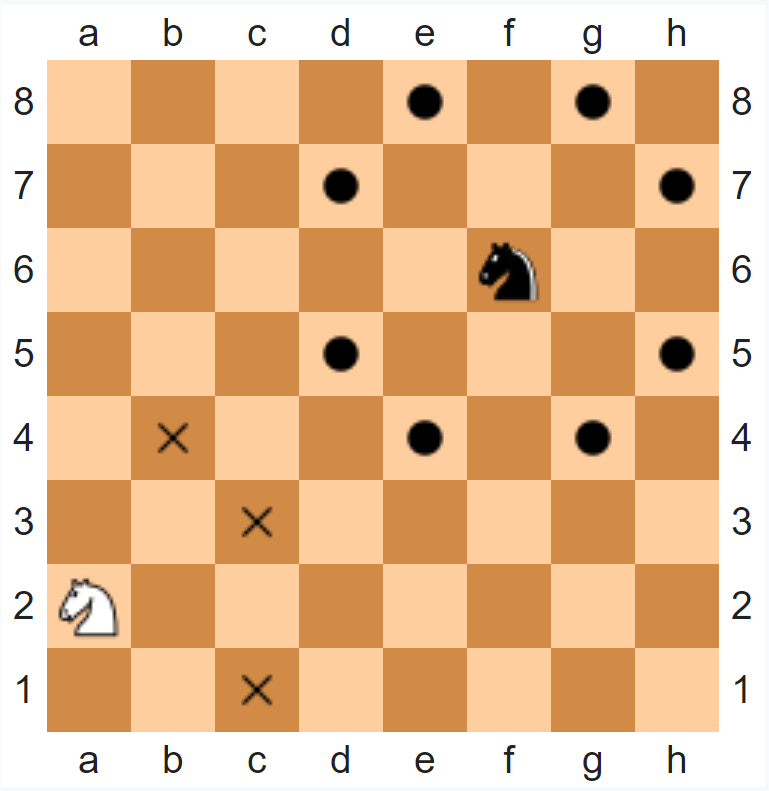
\includegraphics[height=6cm]{mengen/springerzuege.png}
\end{frame}

\begin{frame}{Springerzüge}
	\begin{block}{Aufgabe + Lösung}
		Sei $B = \set{(a, b) \in \N \times \N \mid 1 \leq a \leq 8 \text{ und } 1 \leq b \leq 8}$
		die Formailiserung eines Schachbrettes.
		Das schwarze Feld a1 hat die Koordinaten $(1, 1)$ 
		und das weiße Feld b1 die Koordinaten $(2, 1)$.
		\visible<+(-1)>{}
		\begin{alist}
			\item Geben Sie die Menge $S \subseteq B$ aller schwarzen Felder an, ohne diese erschöpfend aufzuzählen. \\
			\visible<+-|handout:2->{
				$S = \set{(a, b) \in B \mid a + b \text{ ist gerade}}$
			}
			\item Geben Sie die Menge $R \subseteq B \times B$ an, die genau alle möglichen Springerzüge enthält, 
			ohne diese erschöpfend aufzuzählen. \\
			\visible<+-|handout:2->{
				Die Menge 
				$R = \set{((a_1, b_1), (a_2, b_2)) \in B \times B \mid \size{a_1 - a_2} + \size{b_1 - b_2} = 3 \wedge (\size{a_1 - a_2}) \in \set{1, 2}}$
				erfüllt die Bedingung.
			}
			\item Geben Sie die Menge aller Springerzüge, die auf einem schwarzen Feld starten als Mengenausdruck,
			 ohne Klassentermschreibweise (\emph{Set-Comprehension}) zu verwenden. \\
			 \visible<+-|handout:2->{
				$R \cap (S \times B)$
			}
		\end{alist}
	\end{block}
\end{frame}

\section{Binäre Operationen}

\begin{frame}{Definition}
    \begin{block}{Definition}
          Eine \textbf{binäre Operation} auf einer Menge $A$ ist eine Abbildung $\diamond: A \times A \to A$.
    \end{block}
\end{frame}



\begin{frame}{Eigenschaften von binären Operationen}
  \begin{block}{Assoziativ}
    Eine binäre Operation $\diamond: A \times A \to A$ auf einer Menge A heißt \textbf{assoziativ}, wenn für alle $a, b, c \in A$ gilt:
    \begin{center}
        $a \diamond (b \diamond c) = (a \diamond b) \diamond c$
    \end{center}
  \end{block}
  \begin{block}{Kommutativ}
    Eine binäre Operation $\diamond: A \times A \to A$ auf einer Menge A heißt \textbf{kommutativ}, wenn für alle $a, b \in A$ gilt:
    \begin{center}
        $a \diamond b = b \diamond a$
    \end{center}
  \end{block}
\end{frame}

\begin{frame}{Aufgabe 3}
    Auf $\Z \times \Z$ sei eine binäre Operation $\diamond: (\Z \times \Z)^2 \to \Z \times \Z$ wie folgt für alle Paare $(x_1, y_1),(x_2, y_2) \in \Z \times \Z$ definiert:
    \begin{center}
        $(x_1, y_1) \diamond (x_2, y_2) = (x_1 y_2, x_2y_1)$.
    \end{center}
    \visible<+(-1)>{}

    \begin{alist}
        \item Zeigen Sie, dass $\diamond$ nicht kommutativ ist. \\
        \visible<+-|handout:2->{
        $(1,0)\diamond(1,1)=(1,0)\neq(0,1)=(1,1)\diamond(1,0)$
        }
        \item Zeigen Sie, dass $\diamond$ nicht assoziativ ist. \\
        \visible<+-|handout:2->{
        $((1,1)\diamond(1,1))\diamond(1,0)=(1,1)\diamond(1,0)=(0,1)\neq(1,0)=(1,1)\diamond(0,1)=(1,1)\diamond((1,1,)\diamond(1,0))$
        }
        \item Geben Sie eine \textit{unendliche} Menge $K \subset \Z \times \Z$ an, für die folgendes gilt: Wenn $k_1, k_2 \in K$ sind, dann gilt $k_1 \diamond k_2 = k_2 \diamond k_1$ \\
        \visible<+-|handout:2->{
        z.B. $K = \{(x,x)\mid x \in \Z \}$
        }
        \item Beweisen Sie, dass Ihr $K$ die in Teilaufgabe c) verlangte Eigenschaft hat.\\
        \visible<+-|handout:2->{
            Für jede $(x,x),(y,y) \in K$ gilt: $(x,x)\diamond(y,y)=(xy,xy)=(y,y)\diamond(x,x)$.
        }
    \end{alist}
\end{frame}

\section{Wörter}

\begin{frame}{Wörter}
	\begin{block}{Definition}
		\begin{itemize}
			\item Ein \textbf{Alphabet} $A$ ist eine endliche, nichtleere Menge von Zeichen. \pause
			\item Ein \textbf{Wort} $w$  über einem Alphabet $A$ ist ein \textbf{endliche Folge von Zeichen} aus A \\ 
		\end{itemize}
	\end{block}	
	
	\pause
	\begin{block}{Definition}
		$A^*$ ist die \textbf{Menge aller Wörter} beliebiger Länge, die nur Zeichen aus $A$ enthalten.
		% brauchen wir das?
		\mycomment{, also:\\
		\pause 
		$A^*$ ist die Menge aller Abbildungen $w \from \Z_n \functionto B$ mit $n \in \N_0$ und $B \subseteq A$. \\}
	\end{block}

	\pause
	\begin{exampleblock}{Beispiel}
		Sei $ A = \{ \word a, \word b \} $ ein Alphabet. 
		Dann sind $ w_1 = \word{aabbabab}$ und $w_2 = \word{ab} $ zwei mögliche Wörter über $A$. \\
		\impl $ w_1 \in A^*, w_2 \in A^*$
	\end{exampleblock}

\end{frame}

\begin{frame}{Wörter -- \thassedaniel{formal betrachtet}{Formalkram}}
	\begin{block}{Formale Definition}
		Ein \textbf{Wort} $w$  über einem Alphabet $A$ ist eine \textit{surjektive} Abbildung $w \from \Z_n \functionto B$ mit $B \subseteq A$. \\ 
		\smallskip
		Zur Erinnerung: \; $ \Z_n = \{i \in \N_0 \mid 0 \leq i < n \} = \set{0, ..., n-1} $ 
	\end{block}
	
	\begin{exampleblock}{Beispiel}
		Sei $ A := \{ \word a, ..., \word z \} $ ein Alphabet und $B := \set{\word a, \word b, \word e, \word n, \word o, \word r, \word s, \word t} \subseteq A$. \\
		Dann ist ein Wort $w$ gegeben durch $ w \from \Z_{12} \functionto B$, \\ 
		\smallskip
		\begin{tabular}{c|c@{\:}c@{\:}c@{\:}c@{\:}c@{\:}c@{\:}c@{\:}c@{\:}c@{\:}c@{\:}c@{\:}c@{\:}c@{\:}c@{\:}c}
			$i$ & \small 0 & \small 1 & \small 2 & \small 3 & \small 4 & \small 5 & \small 6 & \small 7 & \small 8 & \small 9 & \small 10 & \small 11 \\
			\hline
			$w(i)$ & \word a & \word n & \word a & \word n & \word a & \word s & \word s & \word o & \word r & \word b & \word e & \word t 
		\end{tabular} \\
		\bigskip
		Oder einfach wie vorhin: \quad  $w := \word{ananassorbet}$.
	\end{exampleblock}
\end{frame}

\begin{frame}[t]{Das leere Wort}
	\begin{block}{Definition}
		Wir definieren das \textbf{leere Wort} als $$ \varepsilon \from \Z_0  \functionto \set{} \qquad\text{bzw.}\qquad \eps \from \set{} \functionto \set{} $$ \pause

	\end{block}
	
	\begin{block}{Wichtig}
		Das leere Wort ist \textbf{nicht} Nichts, sondern ein echtes Wort! \\
		($0 \in \N_0$ ist ja auch ne Zahl! $\emptyset$ ist auch ne Menge!)
	\end{block}
		%Wichtig: Das leere Wort ist auch ein \enquote{echtes, gleichberechtigtes} Wort. Die Null ist bei den natürlichen Zahlen ja auch nicht einfach \enquote{nichts}. \medskip \pause
		
		\YesQuestionE{Ist $\eps \from \set{} \functionto \set{} $ eine Relation? Und eine Funktion? Ist es surjektiv?}{
			Achtung: Wir müssen fordern, dass Wörter surjektiv sind, sonst ist das leere Wort nicht eindeutig!
		}
	
\end{frame}


\begin{frame}{Konkatenation von Wörtern}
	\begin{block}{Wörter „aneinanderkleben“}
		Seien $w_1 = \word{erd}, w_2 = \word{blumentopf}$. \\
		Dann ist $ w_1 \* w_2 = \word{erdblumentopf} \neq w_2 \* w_1 = \word{blumentopferd}$. \\ 
		\pause
		Konkatenation ist also \textbf{nicht kommutativ!} \\
		\YesQuestionE{Ist sie \textbf{assoziativ}?}{$(w_1 \* w_2) \* w_3 = w_1 \* (w_2 \* w_3)$.} \medskip 
		\only<+->{Außerdem gilt immer $ \eps \* w \* \eps = w $.}
		
	\end{block}
	
	\pause
	
	\begin{block}{Beobachtung}
		Falls $w=w_1\* w_2 $ und $w_1 \in A^* , w_2 \in B^* $, dann ist
		$ w\in (A \cup B)^* $.
	\end{block}
	
\end{frame}
\begin{frame}{Konkatenation von Wörtern}

	\begin{block}{„Wortpotenzen“}
		\begin{align*}
			w^0 &= \eps \\
			w^k &= \underbrace{w \* w  \cdots  w}_{\text{$k$-mal}}
		\end{align*}

	\end{block}

\end{frame}

\begin{frame}{Länge von Wörtern}
	\begin{block}{Definition}
		$\size w$: Die \textbf{Länge} eines Wortes $w$, also die Gesamtanzahl der Zeichen von $w$.
	\end{block}
	
	\begin{block}{Beispiel}
		$$ \size{\word{hallo}} = 5 \qqquad \size \eps = 0$$
	\end{block}

	\pause
	\begin{block}{Lemma}
		$$ \size{a \* b} = \size a + \size b $$ \\
		\pause
		$$ \size{w^k} = k \* \size w $$
	\end{block}

\end{frame}

\begin{frame}{Wörter}
	\begin{block}{Definition}
		$A^n$: \emph{Menge aller Wörter der Länge $n$} über dem Alphabet $A$.\\
		Wie kann man damit $A^*$ ausdrücken? \\
		\pause
		\[ A^* = \bigcup \limits_{i = 0}^\infty A^i \]
	\end{block}
	
	
	\pause
	\begin{block}{Erinnerung}
		$
		\bigcup \limits_{i\in I} M_i = \{ x \mid \text{es gibt ein } i\in I \text{ so, dass } x\in  M_i \}  
		$
	\end{block}
\end{frame}

\begin{frame}{Aufgabe 4}
	\visible<+(-1)>{}
	\begin{itemize}
		\item Welche Wörter lassen sich aus dem Alphabet $A = \{ \word a , \word b \}$ bilden? Was enthält die Menge $A^*$? \\
		\visible<+-|handout:2->{
			\impl $\word a, \word b, \word {aa}, \word {bb}, \word {ab}, \word {ba}, \word {aaa}, \word {bbb}, \dots$ \\
			\impl $A^*$ enthält genau diese Wörter (und auch $\eps$!).
		}
		\item Ist das Wort $w = \word{aabb} \* \word{ba}$ ein Element der Menge $A^5$? \\
		\visible<+-|handout:2->{
			\impl Nein. $w = \word{aabbba}$ ist zwar ein Wort über $A$, aber hat Länge $6 \neq 5$.
		}
		\item Was ist $A^2 \times A^2$? \\
			\visible<+-|handout:2->{
				\impl $ A^2 \times A^2 = \set{(\word{aa},\word {aa}),(\word{aa},\word{bb}),(\word {aa},\word {ab}),(\word {aa},\word {ba}),(\word {bb},\word {aa}), \dots }$
			} \\ \smallskip
			Wir definieren die Abbildung $f \from A^* \times A^* \functionto A^*, \; (w_1, w_2) \mapsto w_1 \cdot w_2$. \\
			Was ist $f(A^2 \times A^2)$? \\
			\uncover<+-|handout:2->{
				\impl $ f(A^2 \times A^2) = \set{\word{aaaa}, \word{aabb}, \word{aaab}, \word{aaba}, \word{bbaa}, \dots } = A^4 $
			}\\
		\bigskip
		Erinnerung: Für $f \from A \functionto B, M \subseteq A$ definieren wir $f(M) = \{f(a) \mid a \in M\}$
	\end{itemize}
\end{frame}

\begin{frame}{Aufgabe 5}
	Es sei $n \in \N_0$. Wir definieren eine Abbildung $\tau: \Pot (\Z_n) \to A^n$, sodass für $M \in \Pot (\Z_n)$ das Wort $w = \tau(M) \in A^n$ mit $A = \set{0, 1}$ eindeutig durch folgende Eigenschaft gegeben ist: Für jedes $i \in \Z_n$ ist $w(i)=1$ genau dann, wenn $i \in M$ ist.


	\visible<+(-1)>{}
	\begin{alist}
		\item Es sei $n=4$. Geben Sie $\tau(M)$ für jedes $M \in \set{\set{1,2,3},\set{0,3},\set{\emptyset}}$ explizit an. \\
		\visible<+-|handout:2->{
			\impl $\tau(\set{\{1,2,3}) = \word{0111}, \tau(\set{0,3}) = \word{1001},\tau(\set{\{\emptyset}) = \word{0000}$
		}
		\item Es sei $n$ wieder beliebig. Zeigen Sie, dass $\tau$ bijektiv ist. \\
		\visible<+-|handout:2->{
			Injektiv: Seien $M_1, M_2 \in \Pot (\Z_n) mit w = \tau(M_1)=\tau(M_2)$ Dann gilt:
			\begin{center}
				$i \in M_1$ gdw. $w(i) = 1$ gdw. $i \in M_2$
			\end{center}
			Also ist $M_1 = M_2$ und damit $\tau$ injektiv. \\
			Surjektiv: Wir beobachten $\size{\Pot (\Z_n)} = 2^{\size{\Z_n}} = 2^n = \size{A}^n = \size{A^n}$. Somit muss $\tau$ auch surjektiv sein.
		}
		\item Es sei $w \in A^n$. Geben Sie eine hinreichende und notwendige Bedingung für $M \in  \Pot (\Z_n)$ an, sodass $\tau(M)=w$ ist. In Ihrer Formulierung darf dabei $\tau$ nirgends vorkommen. \\
		\visible<+-|handout:2->{
			\impl $M = \set{i \in \Z_n \mid w(i) = 1}$
		}

	\end{alist}
\end{frame}


% Übungsaufgabe 4.1 WS22/23
\begin{frame}{Palindrome}
	Sei $A$ ein Alphabet. Wir betrachten die Funktion $\diamond^R: A* \to A*$,
	die jedem Wort $w \in A*$ seine Spiegelung $w^R \in A$ zuordnet.
	Dieser Operator ist festegelegt für jedes $w \in A$ durch
	\begin{align*}
		\size{w^R} &= \size{w} \\
		w^R(i) &= w(\size{w} - i - 1)	\text{für alle } 0 \leq i \leq \size{w}
	\end{align*}
	Ein Wort $w \in A*$ heißt Palindrom, wenn gilt $w^R = w$. $P_A = \set{w \in A* \mid w = w^R}$
	bezeichnet die Menge aller Palindrome über A.

	\visible<+(-1)>{}
	\begin{alist}
		\item Geben Sie alle Palidrome der Länge 4 über $\set{\word a, \word b}$ an. \\
		\visible<+-|handout:2->{
			$\set{\word{aaaa}, \word{abba}, \word{baab}, \word{bbbb}}$
		}
		\item Betrachten Sie nun die $Q_A = \set{ww^R \mid w \in A*}$ \\
			 Zeigen oder widerlegen Sie $P_A \subseteq Q_A$ \\
		\visible<+-|handout:2->{
			$\word{aba} \in P_A$, aber wegen $\size{\word{aba}} = 3$ nicht in $Q_A$.
		}
	\end{alist}
\end{frame}




\appendix
\beginbackup

\section{Zusammenfassung und Ausblick}

\begin{frame}	
	\begin{block}{Was ihr nun wissen solltet}
		\begin{itemize}
			\item Wie man mit Relationen umgeht
% 			\item Welche Eigenschaften Relationen haben können
% 			\item Was Abbildungen sind und welche Eigenschaften sie haben können
			\item Wie man mit Wörtern rechnet
		\end{itemize}
	\end{block}
	
	\begin{block}{Was nächstes Mal kommt}
		\begin{itemize}
			\item Sinnvollere Gebilde als \word{\thassedaniel{egnarts\sp si\sp efiL}{retsinnaL\sp nosrO}} mit \emph{formalen Sprachen}
			\item Aus Sage wird Logik: \emph{Aussagenlogik}
		\end{itemize}
	\end{block}
\end{frame}

\only<handout:0>{\slideThanks}

\xkcdframe{1121}{Danke für eure Aufmerksamkeit! \smiley}{1.5}

\only<beamer:0>{\slideThanks}

\backupend

\end{document}